\section{Widget}
\label{chap:widget}
\begin{figure}[h]
\centering
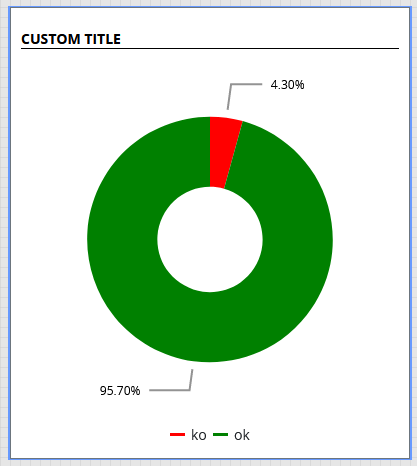
\includegraphics[scale=0.6]{images/widget_example.png}
\end{figure}
\subsection{Composizione}

Un widget è una piccola applicazione, semplice e immediata, che mostra all'utente dati e informazioni, di solito sotto forma di grafici o tabelle. \newline Prendendo ad esempio il pie chart widget si può vedere come un widget lato frontend sia formato da diversi file. La classe contenente i parametri volti alla visualizzazione grafica del widget si chiama \verb|PieChartWidget|. Estende la classe \verb|BaseWidget|, dove viene gestita tutta la logica per la presa dei dati dal backend, ed è decorata con il \verb|WidgetDecorator|, il quale aggiunge ulteriore comportamento al widget.



\begin{lstlisting}[caption={Classe PieChartWidget}, style=javaScriptCode]
@WidgetDecorator({
    endpoint: 'tuple',
    type: WidgetTypeEnum.MOBILITY,
    sourceable: true,
    adapter: PieChartAdapter,
    refreshableInfo: {
        refreshable: true,
    }
})
export class PieChartWidget extends BaseWidget {

    private titleParameter: StringParameter;

    constructor(injector: Injector, widgetDescriptor: WidgetDescriptor) {
        super(injector, widgetDescriptor);
        this.setSize(420, 450);
    }

    public get title(): string {
        return this.titleParameter.value;
    }

    protected createConfigParameters(): Observable<Parameter<unknown>[]> {
        this.createTitleParameter();
        return super.createConfigParameters();
    }

    private createTitleParameter() {
        this.titleParameter = new StringParameter('title', 'Title', 'My title');
        this.titleParameter.longText = 'Title Color';
        this.configParameters.push(this.titleParameter);
    }
}

\end{lstlisting}
Tutta la logica riguardante la visualizzazione dei dati del widget si trova nella classe \verb|PieChartComponent|. Al suo interno viene specificato come la label debba essere mostrata nel pie chart (con il metodo \verb|labelContent|) e viene implementato il metodo \verb|getDataCallback|, richiesto dalla classe \verb|BaseWidgetComponent| che viene estesa da \verb|PieChartComponent|, per salvarsi i dati ogni qualvolta il widget riceva dati dal backend.

\begin{lstlisting}[caption={Classe PieChartComponent}, style=javaScriptCode]
@Component({
    selector: 'app-pie-chart-widget',
    templateUrl: './pie-chart.component.html',
    encapsulation: ViewEncapsulation.None,
    changeDetection: ChangeDetectionStrategy.OnPush
})
export class PieChartComponent extends BaseWidgetComponent<PieChartWidget> {

    public data: TupleData[] = [];
    public backgroundColor = '#ffffff';

    constructor(widgetActions: WidgetActions, injector: Injector) {
        super(widgetActions, injector);
        this.labelContent = this.labelContent.bind(this);
    }

    public labelContent(args: LegendLabelsContentArgs): string {
        return `${args.dataItem.value.toFixed(2)}%`;
    }

    protected getDataCallback(value: any): void {
        this.data = value;
    }
}
\end{lstlisting}
Nel file HTML, di cui viene passato il path al @Component decorator, viene specificato l'aspetto grafico che avrà il widget all'interno della dashboard.

\begin{lstlisting}[caption={File pie-chart.component.html}, style=javaScriptCode]
<aulos-widget-layout [widget]="widget" [backgroundColor]="backgroundColor">
    <aulos-widget-title>
        {{ widget.title }}
    </aulos-widget-title>
    <aulos-widget-content>
        <kendo-chart #customChart [chartArea]="{opacity: 0}">
            <kendo-chart-legend position="bottom"></kendo-chart-legend>
            <kendo-chart-series>
                <kendo-chart-series-item type="donut" [data]="data" field="value" 
                        categoryField="label" colorField="color">
                    <kendo-chart-series-item-labels position="outsideEnd" color="#000" 
                            background="#FFFFFF" [content]="labelContent">
                    </kendo-chart-series-item-labels>
                </kendo-chart-series-item>
            </kendo-chart-series>
        </kendo-chart>
    </aulos-widget-content>
</aulos-widget-layout>
\end{lstlisting}
Infine ogni widget viene incluso in un modulo Angular. All'avvio dell'applicazione il widget viene registrato nel sistema con la chiamata del metodo \verb|registerWidgets|, presente nel modulo. Ciò permette alla dashboard di riconoscere il widget come tale e di mostrarlo selezionabile al momento della configurazione della dashboard.

\begin{lstlisting}[caption={Metodo all'interno del modulo che registra il widget nel sistema}, style=javaScriptCode]
private static registerWidgets(widgetsService: WidgetComponentsService): () => 
    Promise<any> {
        const result = (): Promise<any> => {
            return new Promise((resolve, reject) => {
                const myWidgetDescriptor: WidgetDescriptor = {
                    code: 'pieChartWidgetCode',
                    shortText: 'Pie Chart',
                    longText: 'Descrizione',
                    icon: 'fa fa-pie-chart',
                    group: 'Mobility Group'
                };
                widgetsService.register(myWidgetDescriptor, PieChartWidget, 
                    PieChartComponent);

                resolve();
            });
        };
        return result;
    }
\end{lstlisting}

\subsection{Le classi BaseWidget e BaseWidgetComponent}

Le classi \verb|BaseWidget| e \verb|BaseWidgetComponent| estendono rispettivamente le classi, già presenti nel framework Aulos, \verb|Widget| e \verb|WidgetComponent|. \verb|BaseWidget| e \verb|BaseWidgetComponent| sono classi nate dall'esigenza del progetto di trovare una soluzione per generalizzare il funzionamento dei widget e di rendere la vita più facile ai futuri sviluppatori.
Infatti nelle due classi risiede tutto il comportamento per la raccolta dei dati dal backend, comune a tutti i widget.
All'interno del \verb|BaseWidget| viene iniettato il \verb|WidgetService|, servizio in cui avvengono le chiamate REST, e vengono creati i parametri \verb|source| e \verb|filters|.

\begin{lstlisting}[caption={Creazione dei parametri all'interno della classe BaseWidget}, style=javaScriptCode]
export class BaseWidget extends Widget {

    ...

    private createSourceParameter() {
        this.sourceParameter = new StringParameter('source', 'Source', '');
        this.sourceParameter.longText = 'Source';
        this.sourceParameter.descriptor.editor = new EditorDescriptor(EDITOR_BASE_PATH,
            'SourceEditor');
    }

    private createFiltersParameter() {
        this.filtersParameter = new ContainerParameter('filters', 'Filters', null);
        this.configParameters.push(this.filtersParameter);
    }

}
\end{lstlisting}
Il parametro \verb|source| serve per definire la source a cui chiedere dati, mentre il parametro \verb|filter| si occupa di filtrare la richiesta in base ai filtri presi dal backend e gestiti lato frontend. Il tutto viene inizializzato e caricato tramite il metodo \verb|initSourceCalls|.

\begin{lstlisting}[caption={Inizializzazione dei parametri all'interno della classe BaseWidget}, style=javaScriptCode]
export class BaseWidget extends Widget {
    
    ...
    
    private async initSourceCalls() {
        this.filtersParameter.stateChanges.subscribe(_ => {
            if (this.filtersSet && !this.widgetDTO) {
                this.getData();
            }
        });

        await this.sourceParameter.valueChanges.subscribe(sourceCode => {
            this.sourceSet = true;
            this.widgetService.getSourceProperties(sourceCode).subscribe
            (sourceProperties => {
                this.metadata = sourceProperties.metadata;
                this.setFilters(sourceProperties.filters);
                this.notifyStateChanged();
            });
        });
        this.initSource();
    }

    private getData() {
        if (!this.sourceParameter.value) { return; }
        if (!this.isFiltersReady()) { return; }
        this.widgetService.getData(this.endpoint, this.createRequest()).subscribe
            (value => {
                const data = MetadataService.map(value, this.metadata);
                this.widgetDataSubject.next(data);
        });
    }

    private initSource() {
        this.widgetService.getSource(this.endpoint).subscribe(sourceCode => {
            this.sourceParameter.value = sourceCode;
            this.sourceSet = true;
        });
    }

}
\end{lstlisting}
Nel \verb|BaseWidgetComponent| vi è la sottoscrizione al \verb|dataObservable|, attributo \verb|Observable| fornito da \verb|BaseWidget|, la quale si occupa di chiamare il metodo \verb|getDataCallback| ogni qualvolta vengono presi dati dal backend.
\begin{lstlisting}[caption={Metodi per l'inizializzazione dei dati all'interno della classe BaseWidgetComponent}, style=javaScriptCode]
@Directive()
export abstract class BaseWidgetComponent<T extends BaseWidget> extends 
    WidgetComponent<T> implements OnInit, OnDestroy{

    ...
        
    private initData() {
        this.widget.dataObservable.subscribe(value => {
            if (!value)
                {return;}
            this.getDataCallback(value);
            this.loading = false;
            this.changeDetectorRef.markForCheck();
        });
    }

    protected abstract getDataCallback(value: any): void;
}
\end{lstlisting}

\subsection{Il servizio WidgetService}
Nel \verb|WidgetService| avviene tutta la comunicazione tra frontend e backend.
La sua responsabilità è quella di fare chiamate REST per ottenere i dati da far visualizzare all'interno dei widget. Il principale metodo che si occupa di fare ciò è il metodo \verb|getData| in cui, passatagli una \verb|GenericRequest| composta da un sourceCode e un array di filtri, manda una richiesta POST al backend.

\begin{lstlisting}[caption={Metodo getData all'interno della classe WidgetService}, style=javaScriptCode]
@Injectable({
    providedIn: 'root'
})
export class WidgetService {

    ...

    public getData(widgetUrl: string, genericRequest: GenericRequest): 
        Observable<unknown[]> {
            const adapt = Adapters.getAdapter(widgetUrl);
            const restCall = this.http.post<unknown[]>(`${this.widgetsUrl}/${widgetUrl}`, 
            genericRequest);
            return adapt ? restCall.pipe(map((data) => adapt(data))) : restCall;
        }

}

\end{lstlisting}
Se esiste un'implementazione dell'\verb|Adapter|, interfaccia funzionale con il singolo metodo \verb|adapt|, per quel determinato widget, i dati che verranno presi saranno adattati prima di essere restituiti. In caso contrario verranno passati al widget dati grezzi.

La lista di sources disponibili e la possibile lista di filtri e metadati si ricavano rispettivamente dal metodo \verb|getSources| e dal metodo \verb|getSourceProperties|.

\begin{lstlisting}[caption={Metodi getSources e getSourceProperties all'interno della classe WidgetService}, style=javaScriptCode]
@Injectable({
    providedIn: 'root'
})
export class WidgetService {

    ...
        
    public getSources(widgetUrl: string): Observable<SourceInfo[]> {
        return this.http.get<SourceInfo[]>(`${this.apiUrl}/${widgetUrl}/discovery`);
    }

    public getSourceProperties(sourceCode: string): Observable<SourceProperties> {
        return this.http.get<SourceProperties>(`${this.apiUrl}/filters/${sourceCode}`);
    }

}
\end{lstlisting}
Se un widget è di tipo \verb|MOBILITY|, ovvero legato a dei dati provenienti dalle macchine Loccioni, avrà bisogno della possibilità di filtrare i dati in base alla linea, banco e stazione. Per questo all'interno del \verb|WidgetService| vi sono 3 metodi predisposti per il recupero di questi ultimi.

\begin{lstlisting}[caption={Metodi per recuperare linee, banchi e stazioni all'interno della classe WidgetService}, style=javaScriptCode]
@Injectable({
    providedIn: 'root'
})
export class WidgetService {

    ...
        
    public getLines(sourceCode: string): Observable<number[]> 
    {
        return this.http.get<number[]>(`${this.apiUrl}/topology/${sourceCode}
            /lines`);
    }

    public getBenches(sourceCode: string, lineCode: number): Observable<number[]> 
    {
        return this.http.get<number[]>(`${this.apiUrl}/topology/${sourceCode}
            /benches/${lineCode}`);
    }

    public getStations(sourceCode: string, stationCode: number): Observable<number[]> 
    {
        return this.http.get<number[]>(`${this.apiUrl}/topology/${sourceCode}
            /stations/${stationCode}`);
    }

}
\end{lstlisting}

\subsection{Il decorator factory WidgetDecorator}
Il \verb|WidgetDecorator| ha la responsabilità di aggiungere comportamento a un widget in base alle opzioni passate con l'interfaccia \verb|WidgetOptions|.

\verb|WidgetOptions| ha la seguente struttura:

\begin{lstlisting}[caption={Struttura delle WidgetOptions e delle RefreshableInfo}, style=javaScriptCode]
export interface WidgetOptions {
    // indicates which endpoint the widget has to use to take data from
    endpoint: string;
    // indicates the widget type (currently IT/MOBILITY)
    type: WidgetTypeEnum;
    // indicates whether or not the widget has a selectable source parameter
    sourceable?: boolean;
    /* indicates whether or not the widget has a refresh parameter and can be 
    used to set the default refresh rate*/
    refreshableInfo?: RefreshableInfo; 
    /* indicates the adapter class used to transform received data into a 
    more useful form*/
    adapter?: any;
}

export interface RefreshableInfo {
    refreshable: boolean;
    defaultRefreshRate?: RefreshRateEnum;
}
\end{lstlisting}
Il comportamento viene aggiunto al widget tramite altri decorators verificando le opzioni passate al momento della decorazione.

\begin{lstlisting}[caption={Decorator factory WidgetDecorator}, style=javaScriptCode]
export const WidgetDecorator: (options: WidgetOptions) => (target: Function) => 
    void = (options: WidgetOptions) => {

    return (target: Function) => {
        target.prototype.baseWidgetDecorator = true;
        target.prototype.endpoint = options.endpoint;

        switch (options.type) {
            case WidgetTypeEnum.IT:
                break;
            case WidgetTypeEnum.MOBILITY:
                Mobility(target);
                break;
        }
        if (options.sourceable) {
            Sourceable(target);
        }
        if (options.refreshableInfo?.refreshable) {
            Refreshable({defaultRefreshRate: options.refreshableInfo
                .defaultRefreshRate})(target);
        }

        if (options.adapter) {
            const adaptFunc = options.adapter.prototype.adapt;
            if (adaptFunc) {
                Adapters.setAdapter(target.prototype.endpoint, adaptFunc);
            }
        }
    };
};
\end{lstlisting}
\subsection{Mobility Decorator}
Il \verb|Mobility| decorator si occupa di aggiungere i parametri atti al filtraggio dei dati di un widget in base alla linea, banco e stazione.

\begin{lstlisting}[caption={Metodo di creazione dei parametri all'interno del decorator Mobility}, style=javaScriptCode]
export const Mobility: (target: Function) => void = (target: Function) => {

    ...

    target.prototype.createTopologyParameters = function(...args) {
        target.prototype.lineCodeParameter = new NumberParameter('lineCode', 
            'Line Code', 0);
        target.prototype.benchCodeParameter = new NumberParameter('benchCode', 
            'Bench Code', 0);
        target.prototype.stationCodeParameter = new NumberParameter('stationCode', 
            'Station Code', 0);

        this.lineCodeParameter.descriptor.editor = new EditorDescriptor(
            EDITOR_BASE_PATH, 'DropdownEditor', []);
        this.benchCodeParameter.descriptor.editor = new EditorDescriptor(
            EDITOR_BASE_PATH, 'DropdownEditor', []);
        this.stationCodeParameter.descriptor.editor = new EditorDescriptor(
            EDITOR_BASE_PATH, 'DropdownEditor', []);

        this.configParameters.push(this.lineCodeParameter);
        this.configParameters.push(this.benchCodeParameter);
        this.configParameters.push(this.stationCodeParameter);
    };

};
\end{lstlisting}
Il metodo che inizializza e definisce il comportamento che il widget avrà al cambio di uno dei parametri è il metodo \verb|initTopology|.

\begin{lstlisting}[caption={Metodo initTopology all'interno del decorator Mobility}, style=javaScriptCode]
export const Mobility: (target: Function) => void = (target: Function) => {

    ...

    target.prototype.initTopology = function(...args) {
        if (this.sourceSet) {
            this.getLines(this.sourceParameter.value, this);
        }
        this.sourceParameter.valueChanges.subscribe(sourceCode => {
            this.getLines(sourceCode, this);
        });

        this.lineCodeParameter.valueChanges.subscribe(lineCode => {
            this.resetBench(this);
            this.getData(this);
            if (this.sourceParameter.value) {
                this.widgetService.getBenches(this.sourceParameter.value, lineCode)
                    .subscribe(benchCodes => {
                    this.benchCodes = benchCodes;
                    this.benchCodeParameter.descriptor.editor.options = benchCodes;
                    this.benchCodeParameter.notifyStateChanged();
                });
            }
        });

        this.benchCodeParameter.valueChanges.subscribe(benchCode => {
            this.resetStation(this);
            this.getData(this);
            if (this.sourceParameter.value) {
                this.widgetService.getStations(this.sourceParameter.value, benchCode)
                    .subscribe(stationCodes => {
                    this.stationCodes = stationCodes;
                    this.stationCodeParameter.descriptor.editor.options = stationCodes;
                    this.stationCodeParameter.notifyStateChanged();
                });
            }
        });

        this.stationCodeParameter.valueChanges.subscribe(_ => {
            this.getData(this);
        });
    };

};
\end{lstlisting}

\subsection{Sourceable decorator}
Il \verb|Sourceable| decorator dà al widget la possiblità di far selezione all'utente la source dove prendere i dati dal backend.

Ogni widget che estende \verb|BaseWidget| ha al suo interno il parametro \verb|SourceParame|-\verb|ter|. Nel \verb|baseWidget| \verb|initSource| si occupa di impostare l'unica source da cui il widget prenderà i dati, mentre con l'override all'interno del \verb|Sourceable| decorator il metodo ha lo scopo di impostare la source in base a ciò che selezionerà l'utente.

\begin{lstlisting}[caption={Metodo initSource e override}, style=javaScriptCode]
export class BaseWidget extends Widget {
    
    ...
    
    private initSource() {
        this.widgetService.getSource(this.endpoint).subscribe(sourceCode => {
            this.sourceParameter.value = sourceCode;
            this.sourceSet = true;
        });
    }
    
}


export const Sourceable = (target: Function) => {

    ...

    target.prototype.initSource = function() {
        this.sourceParameter.valueChanges.subscribe(sourceCode => {
            this.sourceParameter.value = sourceCode;
        });
    };

};
\end{lstlisting}
La configurazione delle possibili source disponibili avviene nell'override del metodo \verb|initSourceCalls|. Le \verb|options| per l'\verb|editor| del \verb|sourceParameter| vengono impostate con il metodo \verb|setSources|.

\begin{lstlisting}[caption={Metodo setSources e override del metodo initSourceCalls all'interno del Sourceable Decorator}, style=javaScriptCode]
export const Sourceable = (target: Function) => {

    ...
    
    const oldInitSourceCalls = target.prototype.initSourceCalls;
    target.prototype.initSourceCalls = function() {
        this.widgetService.getSources(target.prototype.endpoint).subscribe(sources => {
            this.setSources(sources);
        });
        if (oldInitSourceCalls){
            oldInitSourceCalls.apply(this);
        }
    };

    target.prototype.setSources = function(sources: SourceInfo[]) {
        this.sourceParameter.descriptor.editor.options = sources;
    };

};
\end{lstlisting}
\subsection{Refreshable decorator}
Il \verb|Refreshable| decorator permette al widget di aggiornarsi e ricaricare i dati ad uno specifico intervallo di tempo. Il valore di default dell'intervallo può essere cambiato passando all'interno delle \verb|RefreshableInfo| anche un \verb|defaultRefreshRate|.
L'intervallo poi potrà essere selezionato dall'utente al momento di configurazione della dashboard grazie al \verb|refreshRateParameter| che viene aggiunto al widget.

\begin{lstlisting}[caption={Creazione del refreshRateParameter all'interno del Refreshable decorator}, style=javaScriptCode]
export const Refreshable: (options?: RefreshableOptions) => (Function) => 
    void = (options?: RefreshableOptions) => {
    return (target: Function) => {
        
        ...
        
        target.prototype.createRefreshParameter = function() {
            target.prototype.refreshRateParameter = new NumberParameter('refreshRate', 
                'Refresh Rate', this.defaultRefreshRate);
            this.refreshRateParameter.descriptor.editor = new EditorDescriptor(
                EDITOR_BASE_PATH,
                'EnumEditor',
                this.generateDefaultEnumOptions());
            this.configParameters.push(this.refreshRateParameter);
        };
        
    };
};
\end{lstlisting}
Ogni qualvolta un utente cambi intervallo di refresh viene effettuata una nuova registrazione all'Observable presente nel \verb|RefreshService|, legato a quel determinato intervallo, e viene annullata la precedente registrazione.

\begin{lstlisting}[caption={Metodo updateSubscription all'interno del Refreshable decorator}, style=javaScriptCode]
export const Refreshable: (options?: RefreshableOptions) => (Function) => 
    void = (options?: RefreshableOptions) => {
    return (target: Function) => {
        
        ...

        target.prototype.updateSubscription = function(refreshRate: number) {
            if (this.subscription) { this.subscription.unsubscribe(); }
            this.subscription = this.refreshService.getObservableOfInterval(refreshRate)
                .pipe(
                    exhaustMap(() => { this.getData(); return EMPTY; })
                )
                .subscribe();
        };
        
    };
};
\end{lstlisting}
Il \verb|RefreshService| ha la responsabilità di tenere salvati gli Observable legati a tutti gli intervalli richiesti.

\begin{lstlisting}[caption={Classe RefreshService}, style=javaScriptCode]
@Injectable({
  providedIn: 'root'
})
export class RefreshService {

  private intervals: Map<number, Observable<any>> = new Map();
  constructor() { }

  public getObservableOfInterval(refreshRate: number): Observable<any> {
    if (!this.intervals.has(refreshRate)) {
      this.intervals.set(refreshRate, interval(refreshRate).pipe(
        multicast(new Subject()),
        refCount()
      ));
    }
    return this.intervals.get(refreshRate);
  }
}
\end{lstlisting}
Nello specifico il metodo \verb|getObservableOfInterval| ritorna l'Observable dell'intervallo di tempo fornito. Se l'intervallo non è presente all'interno di \verb|intervals| allora lo inserisce creando l'Observable legato ad esso.

L'\verb|Observable| viene creato con il metodo \verb|interval|, il quale crea un \verb|Observable| che emette numeri sequenziali all'intervallo di tempo specificato. Poi viene trasformato con il metodo \verb|multicast| in un \verb|ConnectableObservable|, particolare tipo di \verb|Observable| che non emetterà valori finché non sarà chiamato il metodo \verb|connect|. Questa chiamata viene resa automatizzata grazie al metodo \verb|refCount|, il quale gestisce la connessione in modo tale da mantenerla attiva fintanto ci siano observer in ascolto.

\begin{lstlisting}[caption={Classe RefreshService}, style=html]
<aulos-editor-layout [editorConfiguration]="editorConfiguration">
  <ng-template aulosEditorSmallTemplate>
    <div class="input-group" [class.hidden]="disabled">
      <input type="text" 
        class="form-control form-control-sm is-invalid"
        [placeholder]=mySelection[0] ? mySelection[0] : 
        'Choose data source...'  | aulosTranslate 
        disabled readonly>
      <button class="btn btn-sm btn-icon" [disabled]="disabled" (click)="showExpandedModal()">
        <i class="fontaulos fontaulos-edit"></i>
      </button>
    </div>
  </ng-template>
  <ng-template aulosEditorCompactTemplate>
    <div class="input-group" [class.hidden]="disabled">
      <input 
      type="text" 
      class="form-control is-invalid" 
      [placeholder]="this.model.value ? 
      this.model.value : 
      'Choose data source...'  | aulosTranslate" 
      disabled
        readonly>
      <button class="btn btn-icon" [disabled]="disabled" (click)="showExpandedModal()">
        <i class="fontaulos fontaulos-edit"></i>
      </button>
    </div>
  </ng-template>
  <ng-template aulosEditorExpandedTemplate>
    <kendo-grid
              [data]="gridData"
              [style.maxlength]="501"
              [filterable]="true"
              [filter]="state.filter"
              [selectable]="selectableSettings"
              [sortable]="true"
              style="padding-top: 2%; padding-bottom: 5%;"
              (dataStateChange)="dataStateChange($event)"
              kendoGridSelectBy="sourceCode"
              [selectedKeys]="tmpSelection"
            >
            <kendo-grid-checkbox-column width="60%"></kendo-grid-checkbox-column>
            <kendo-grid-column field="sourceCode" filter="text"></kendo-grid-column>
            <kendo-grid-column field="shortText" filter="text"></kendo-grid-column>
            <kendo-grid-column field="longText" filter="text"></kendo-grid-column>
            <ng-template kendoGridNoRecordsTemplate>
              No sources available.
           </ng-template>
          </kendo-grid>
  </ng-template>
</aulos-editor-layout>
\end{lstlisting}